\tableofcontents
\newpage

\section*{前言}
\addcontentsline{toc}{section}{前言}
欢迎各位大朋友,小朋友来到丰富多彩的网络世界!在网上冲浪乃至学习生活中,我们都需要一些基本的信息素养。这本小册子就是为了帮助大家提高信息素养而写的。希望大家能够从中受益。

如果你觉得自己知道的不多,请按照顺序一节一节阅读并照着做。如果你觉得自己挺懂的,可以选感兴趣的部分阅读。在每个小节前面我会用一些图标标识出本小节内容所需要的前提条件,有些图标可以点击并跳转到对应的部分。
此处先对各种图标做一个解释:
\begin{itemize}
    \item \hyperlink{warp}{\faIcon{globe}}\quad 国际互联网
    \item \hyperlink{mail}{\faIcon{mail-bulk}}\quad 国外邮箱帐号
    \item \faIcon{alipay}\quad 支付宝
    \item \faIcon{bitcoin}\quad 虚拟货币
    \item \hyperlink{sms-code}{\faIcon{sim-card}}\quad 国外手机号码
    \item \hyperlink{card}{\faIcon{credit-card}}\quad 虚拟信用卡
    \item \hyperlink{gift-card}{\faIcon{app-store-ios}}\quad \textsf{App Store}礼品卡
    \item \hyperlink{google}{\faIcon{google}}\quad \textsf{Google}帐号
    \item \hyperlink{github}{\faIcon{github}}\quad \textsf{Github}帐号
    \item \hyperlink{api}{\faIcon{code}}\quad API Key
\end{itemize}

\hypertarget{mail}{\section*{邮箱准备}}
\addcontentsline{toc}{section}{邮箱准备}
邮箱是在网上冲浪所必需的。有小朋友可能会问,我有\textsf{QQ}邮箱或者\textsf{163}邮箱了,是不是可以直接跳过这一章了?答案是否定的。许多网站和服务都不支持国内的邮箱,你需要准备国外的邮箱。
你可以在点击链接 \href{https://signup.live.com/signup}{\color{black}\faLink} 注册一个 \textsf{Outlook} 邮箱,很快就会用上的。

\section{信息源的选择}
\vspace{3cm}
\begin{quote}{\small \ 知乎提问:中文互联网的产出在渐渐枯萎吗?\normalsize}
    \Huge{“}
    \normalsize \texttt{简中互联网已经成为垃圾堆。}
    \end{quote}
    
\vspace{3cm}
信息源是我们获取信息的基础。百度搜索,百度百科,\textsf{CSDN}等常见的中文网站并不是好的选择。它们往往充斥着浓重的商业气息和不规范转载,低水平甚至误导人的文章泛滥成灾。
与其屎里淘金,不如转而用一些相对更好的网站:\textsf{Google}, \textsf{Stackoverflow}, \textsf{Github}等等。但是这些网站基本都使用英语,所提升自己的英语能力十分\sout{甚至九分}重要。
如果你感兴趣了解更多,可以访问链接 \href{https://web.archive.org/web/20220321083337/https://www.zhihu.com/question/49684783/answer/2305132342}{\color{black}\faLink} 
阅读上面引用的原文存档(访问需要 \hyperlink{warp}{\faIcon{globe}})。

\newpage
\section{Scientific上网}

\vspace{1cm}
\begin{quote}{\small \ 墨菲斯,尼布甲尼撒号船长\normalsize}
    \Huge{“}
    \normalsize \texttt{我只能带你到这扇门,你必须自己走进去。}
    \end{quote}
\vspace{1cm}

众所周知,上文所述相对更好的网站在正常情况下很多是无法打开的。所以,我们需要有一些办法来访问这些网站。最简便的办法是使用\textsf{Cloudflare}公司的\textsf{1.1.1.1}应用。
\hypertarget{warp}{\subsection{1.1.1.1}}
点击链接 \href{https://one.one.one.one}{\color{black}\faLink},选择对应你所使用的设备的版本下载并安装。确认开关上方的字是“WARP”,打开开关,看见“Connected. Your Internet is private.”字样即表明连接成功。

\begin{figure}[h]
    \centering
    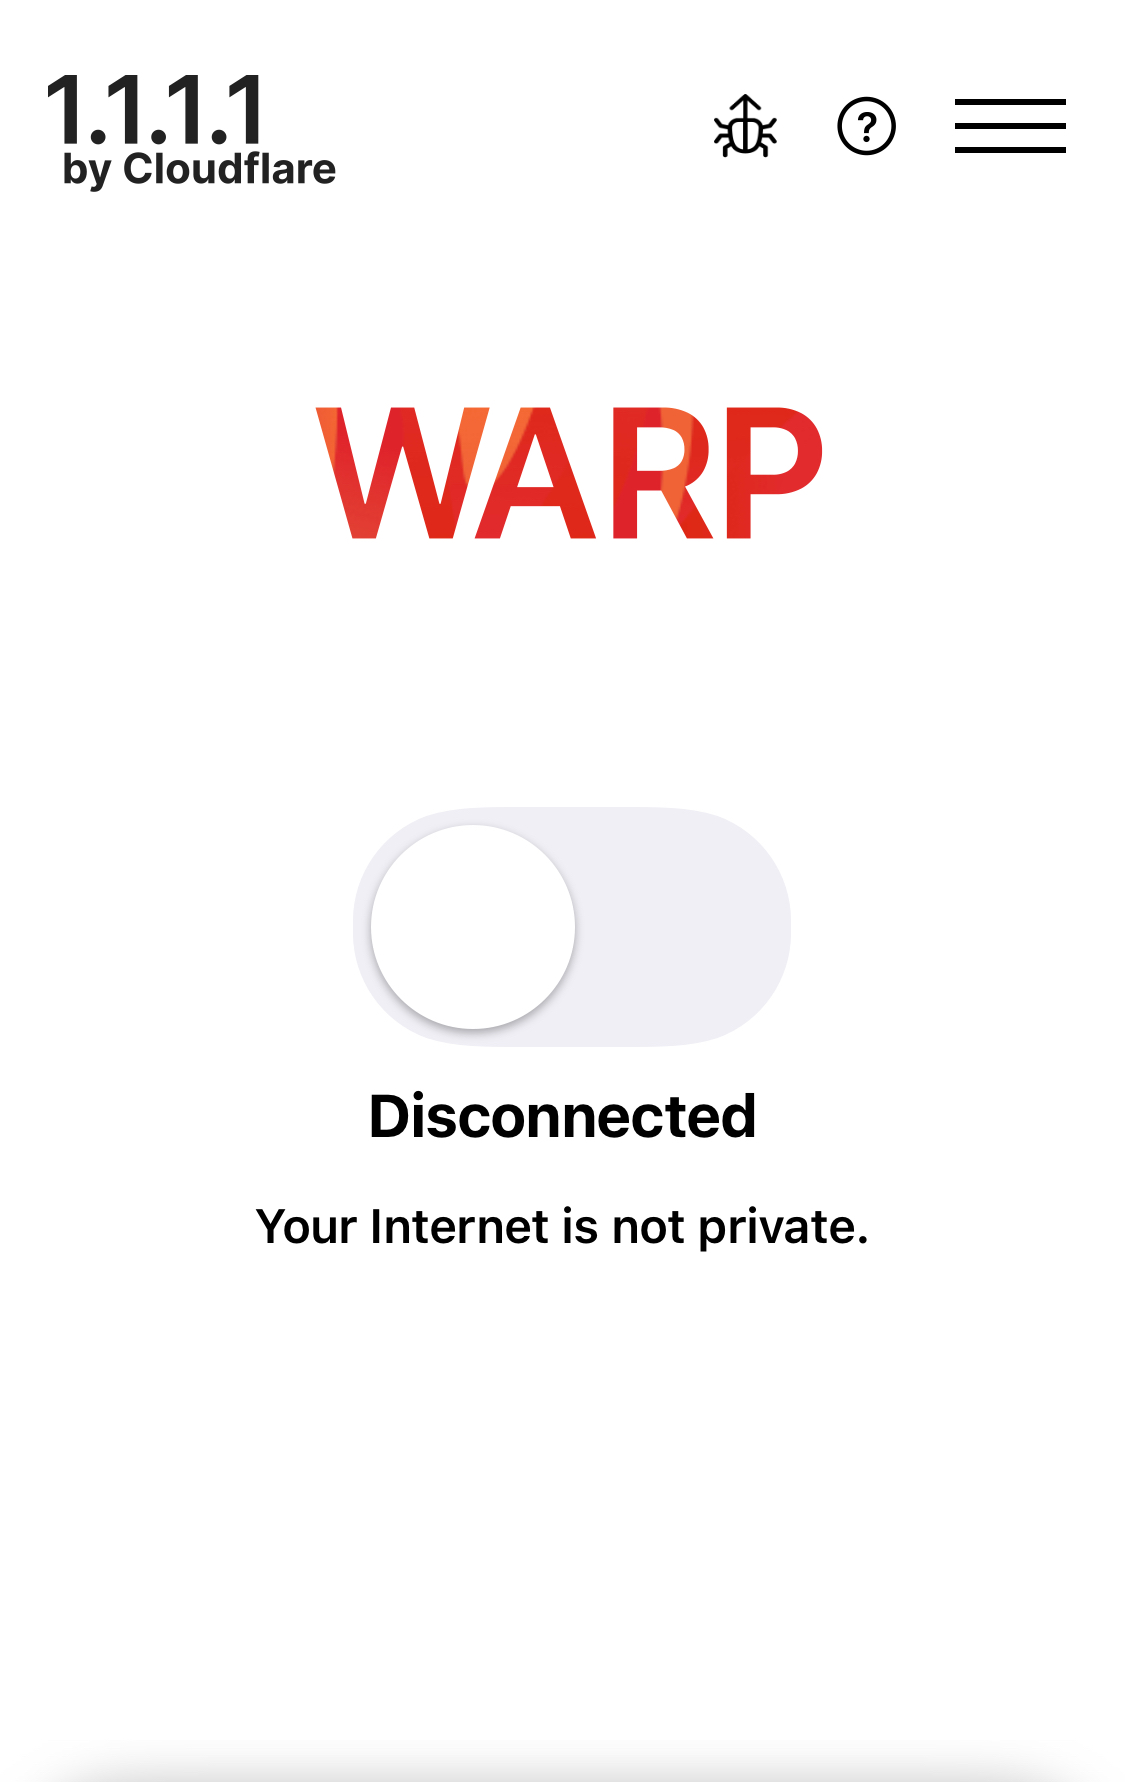
\includegraphics[width=0.4\columnwidth]{pics/warp.jpg}
    \caption{\textsf{1.1.1.1}应用界面,以\textsf{\textsf{iOS}}为例}
\end{figure}

现在点击链接 \href{https://google.com}{\color{black}\faLink} 便可以访问\textsf{Google}了。然而,\textsf{WARP}也有其局限性。例如在访问国内网站的时候会比较卡,或者被部分网站拦截等等。
因此WARP一般只作为备用方案,我们需要更好的工具。
\subsection{代理供应商\&代理软件}
代理供应商(俗称“机场”)与代理软件是实现网络代理(或科学上网)的核心工具。它们能够帮助用户通过中转服务器访问被屏蔽的网站或服务。
常见的代理软件包括 \textsf{Clash}、\textsf{V2RayN}、\textsf{Shadowrocket}、以及 \textsf{Singbox} 等。

代理供应商提供的服务通常分为不同套餐,通常需要花钱订阅,你可以根据带宽、速度和流量的需求进行选择。当你购买订阅后,会获得一个“订阅地址”。
把导入地址至代理软件便可加密和转发所有(或部分)网络流量,实现更高效地科学上网。

\subsubsection{安装代理软件}
\roundedbox{\color{RedOrange}{\textsf{必须:}\hyperlink{warp}{\faIcon{globe}}} }

此处以\textsf{Clash Verge Rev}(后文简称\textsf{Clash})为例介绍。访问本项目仓库(Repository)的Release页面链接 \href{https://github.com/clash-verge-rev/clash-verge-rev/releases/tag/v1.7.7}{\color{black}\faLink} 
选择对应你所使用的设备的版本下载并安装。安装完毕后打开软件备用。

\subsubsection{选择一个(或多个)机场}
\roundedbox{\color{RedOrange}{\textsf{必须:}\hyperlink{warp}{\faIcon{globe}} \hyperlink{mail}{\faIcon{mail-bulk}} } \color{Melon}{\textsf{可选:}\faIcon{alipay} \faIcon{bitcoin}}}

市面上有数量不少的机场可以选择,可以自行搜索或者访问链接 \href{https://github.com/hwanz/SSR-V2ray-Trojan}{\color{black}\faLink},
选择自己认为合适的(建议:不要买年付或者季付,以免机场跑路)。笔者使用的是 \href{https://mojie.me}{\color{black}\faLink},主要看重这家是按量付费而非按时间订阅。

注册机场需要使用邮箱,最好选择国外邮箱(例如上文提到的\textsf{Outlook})。通常机场都支持使用支付宝或者微信支付。购买完成后你可以寻找机场网站上的使用文档将订阅链接导入到\textsf{Clash}中,通常有一键导入的选项。

\subsubsection{配置代理软件}

导入完成后,你就可以退出\textsf{Cloudflare}的\textsf{1.1.1.1}软件了。现在到\textsf{Clash}的设置中打开“系统代理”、“开机自启”和“静默启动”。接下来的日子里就不要关闭\textsf{Clash}了。
\begin{figure}[H]
    \centering
    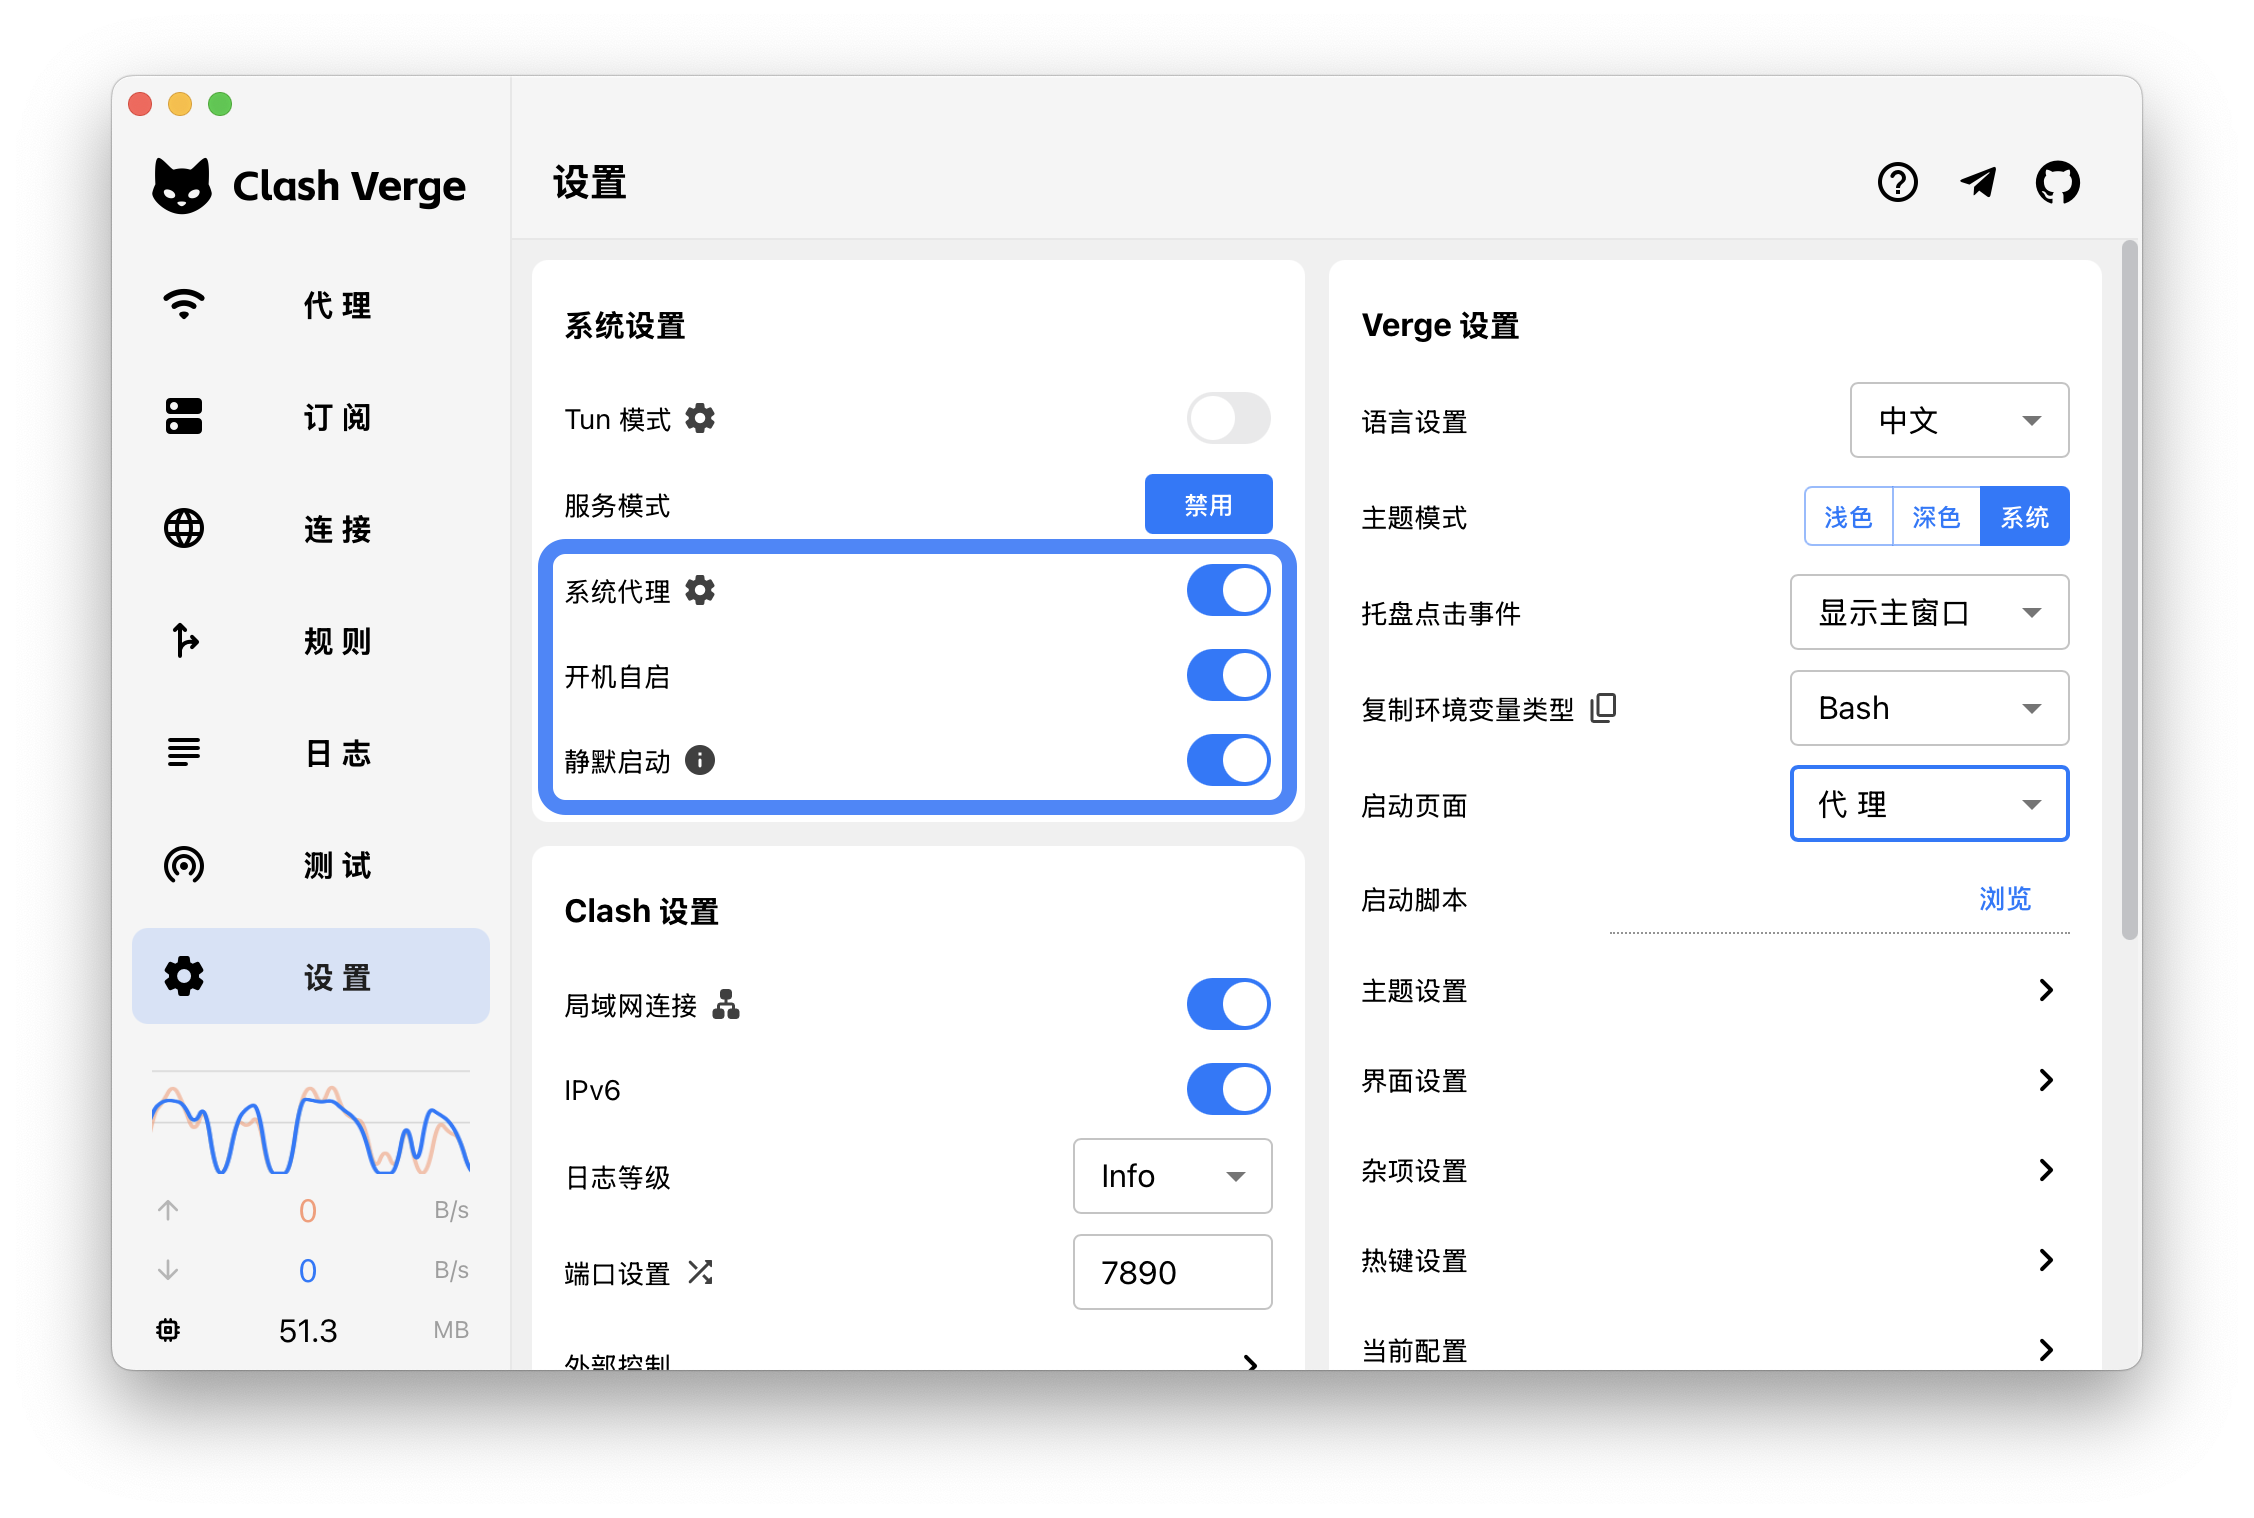
\includegraphics[width=0.8\textwidth]{pics/clash-settings.png}
    \caption{\textsf{Clash}设置界面}
\end{figure}
%\FloatBarrier 

进入\textsf{Clash}的“代理”界面。你可以看到如下的设计。

\begin{figure}[H]
    \centering
    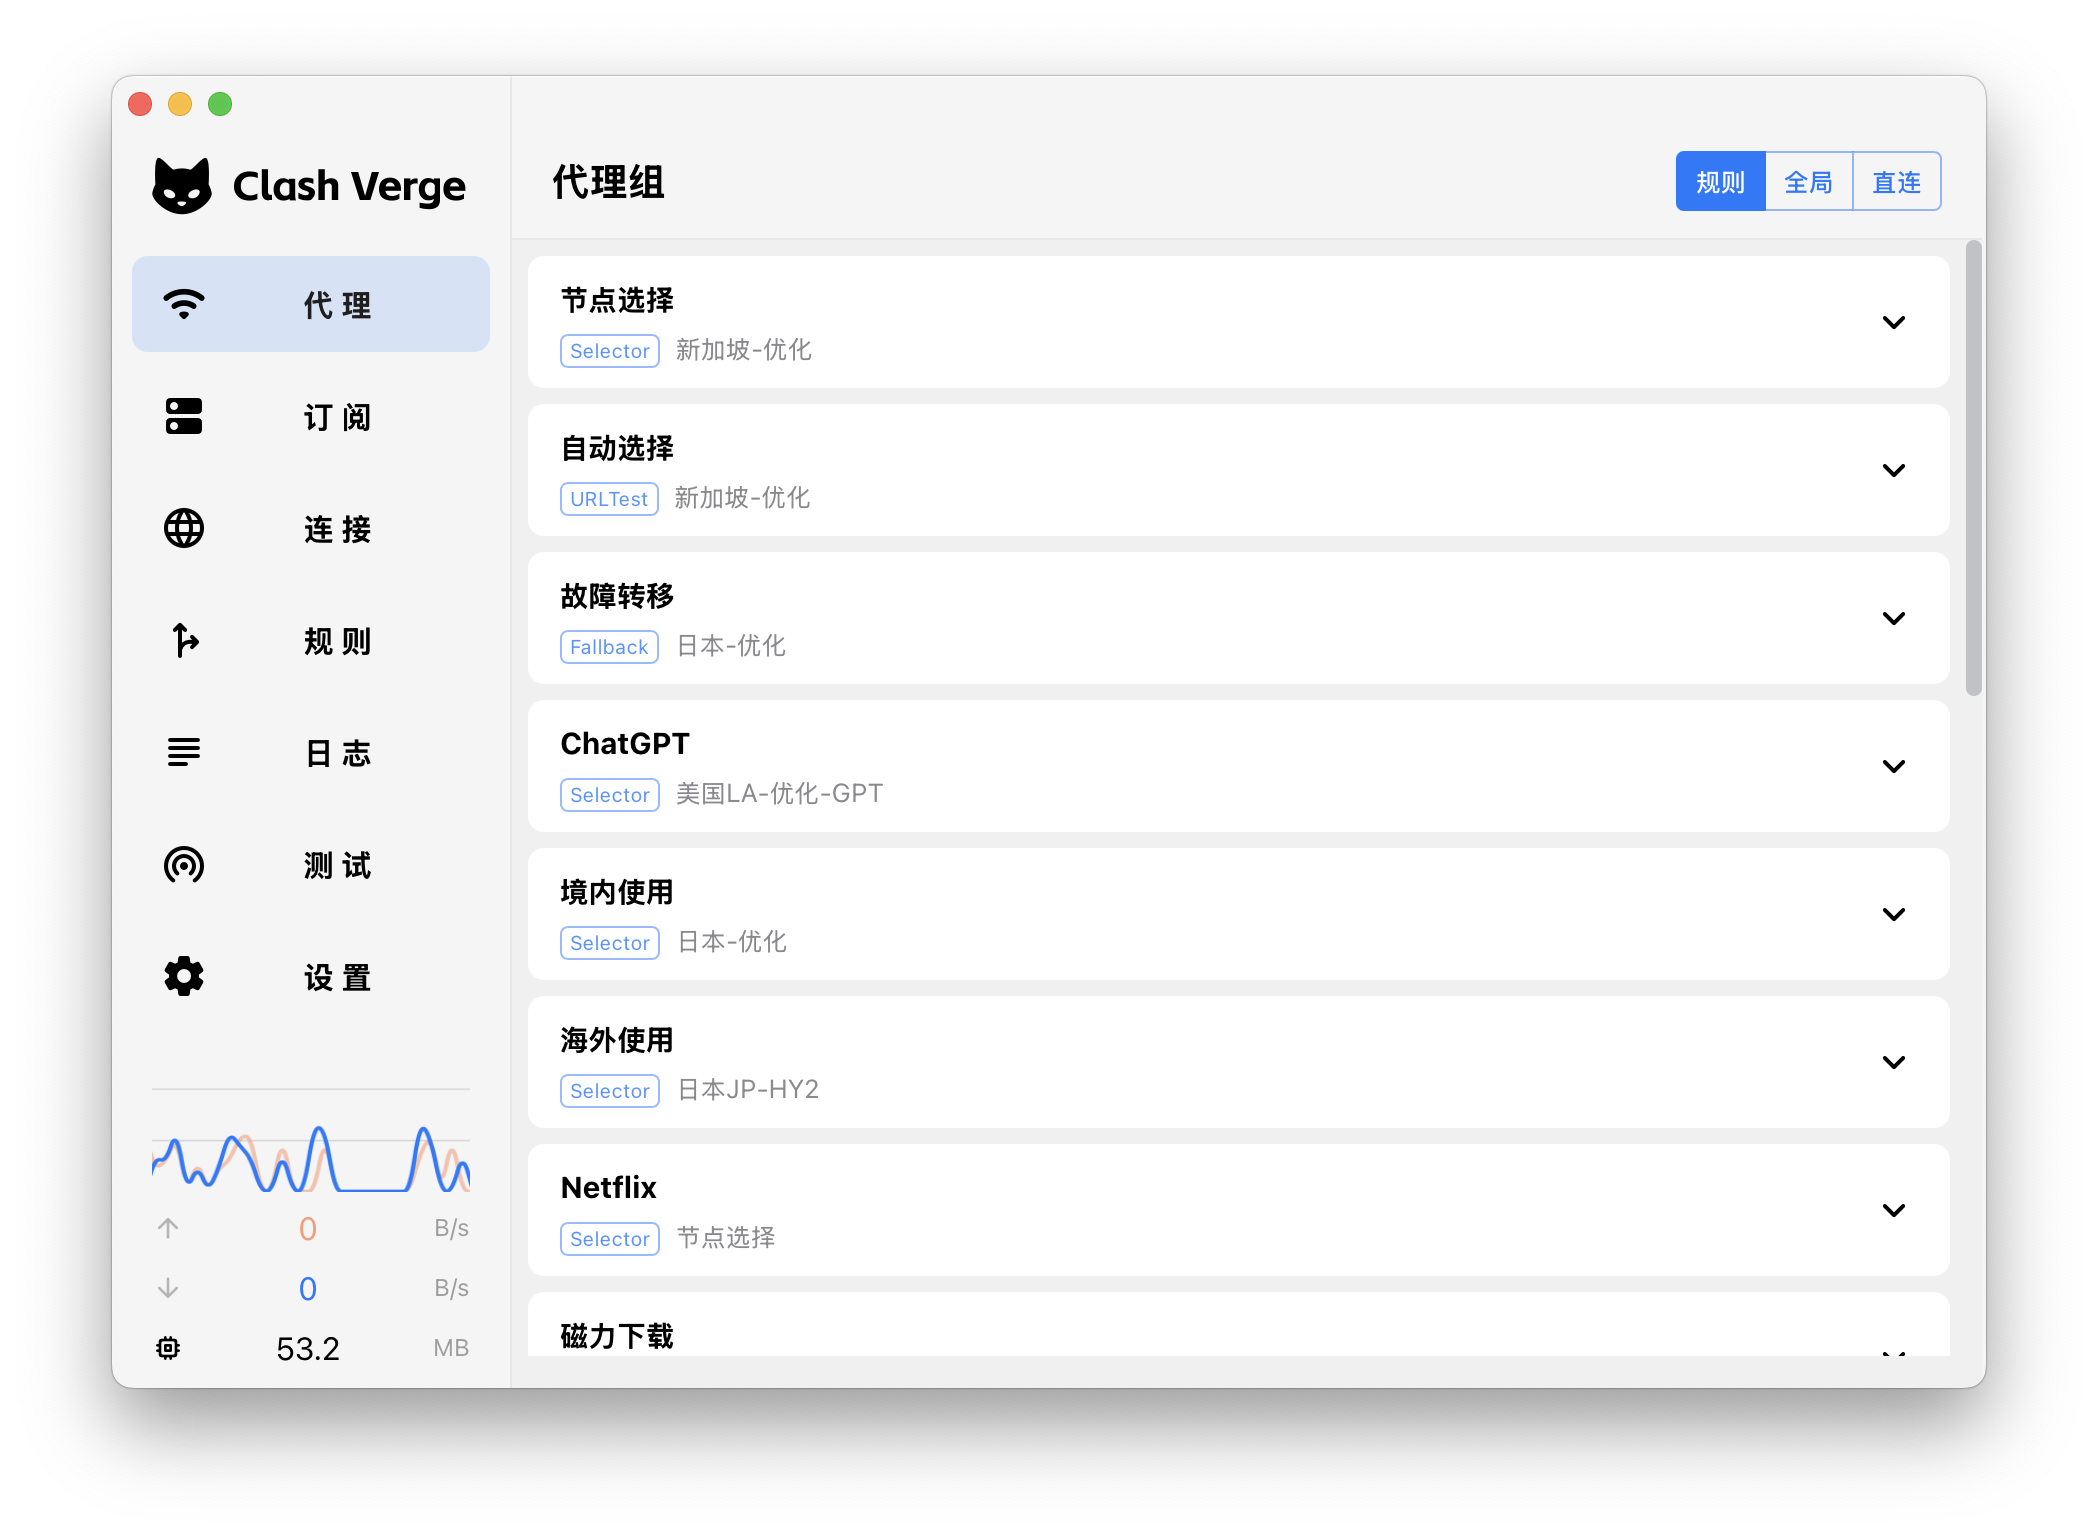
\includegraphics[width=0.8\textwidth]{pics/clash-proxy.png}
    \caption{\textsf{Clash}代理界面}
\end{figure}

这里的每个选项都是针对不同流量的代理方案。点开最上方的选项,图中是“节点选择”,选一个你喜欢的代理服务器(如果你不知道怎么选择,可以先点一下Wifi形状的图标测速,选一个比较快的)。

注意右上角要选择“规则”(如果你选了全局,那所有流量都走代理,会导致国内网站访问过慢和流量消耗过快;如果你选了直连,那就相当于没有安装\textsf{Clash})。

恭喜你可以畅游国内与国际互联网了!

\section{\textsf{Google}与\textsf{Github}帐号准备}
\subsection{为什么需要准备这两个帐号}
很多在线服务(比如\textsf{Gmail}、\textsf{Google Drive}、\textsf{YouTube}等)和第三方工具都与\textsf{Google}帐号集成,方便快捷地登录。
而\textsf{GitHub}是目前最流行的代码托管和版本控制平台,尤其对于编程和开发工作非常有用。拥有\textsf{GitHub}帐号,你可以方便地管理代码、参与开源项目、托管个人项目甚至是简历,适用于开发者或学习编程的同学。
\subsection{如何注册\textsf{Google}和\textsf{GitHub}帐号}
\roundedbox{\color{RedOrange}{\textsf{必须:}\hyperlink{warp}{\faIcon{globe}} \hyperlink{mail}{\faIcon{mail-bulk}}} }

\begin{itemize}
    \item \hypertarget{google}{\textsf{Google}帐号}:只需前往\textsf{Google}的网站 \href{https://accounts.google.com}{\color{black}\faLink},根据提示输入个人信息,如姓名、邮箱、密码等,即可完成注册。
    \item \hypertarget{github}{\textsf{GitHub}帐号}:可以前往\textsf{GitHub}的官网 \href{https://github.com}{\color{black}\faLink},点击“Sign up”并按照步骤填写用户名、邮箱、密码等信息,完成注册。如果你是大学生,那就更好了。你可以申请\textsf{Github Education},免费使用\textsf{Copilot}。
\end{itemize}

\subsubsection*{帐号安全}
你可以结合\textsf{Passkey},双重验证 (\textsf{2FA})与密码管理器来保证你帐号的安全性,一般在帐号的安全设置页面可以找到这些选项。这是十分重要的,务必不要忽视。

\section{在线语言模型的使用}

大语言模型,也称LLM (Large Language Models),就是基于大量数据进行预训练的超大型深度学习模型。最名震遐迩的莫过于\textsf{ChatGPT}了。本章节将带领大家上手一些最强大的LLM。

\subsection{\textsf{ChatGPT}}
\roundedbox{\color{RedOrange}{\textsf{必须:}\hyperlink{warp}{\faIcon{globe}} \hyperlink{mail}{\faIcon{mail-bulk}} \hyperlink{sms-code}{\faIcon{sim-card}}} \color{Melon}{\textsf{可选:}\hyperlink{card}{\faIcon{credit-card}} \hyperlink{gift-card}{\faIcon{app-store-ios}}}}

\begin{quote}{续下文}
    \Huge{“}
    \normalsize \texttt{ChatGPT总体上和一个本科生-研究生的常识相符,但大部分的GPT版本,比较机械,看不出有特别的人格特质,通常你用什么水平的词,它也会跟着你的水平输出,遇强则强,遇弱则弱,但不太会有人格特征,它的角色大部分时候只是一台问答机。它的频响曲线就很哈曼的那种。}
\end{quote}


\textsf{OpenAI}公司开发的模型。点击链接 \href{https://chatgpt.com}{\color{black}\faLink},就进入了\textsf{ChatGPT}的网站。在不登录的情况下只能使用\textsf{4o-mini}模型,所以需要注册帐号使用更强大的\textsf{GPT-4o}。点击右上角的Sign Up以注册。

注册过程中,可能会需要验证手机号码,但是这里是不支持中国大陆(+86)的手机号的,这时就要用到接码平台 \hyperlink{sms-code}{\faIcon{share}}了。

\begin{figure}[H]
    \centering
    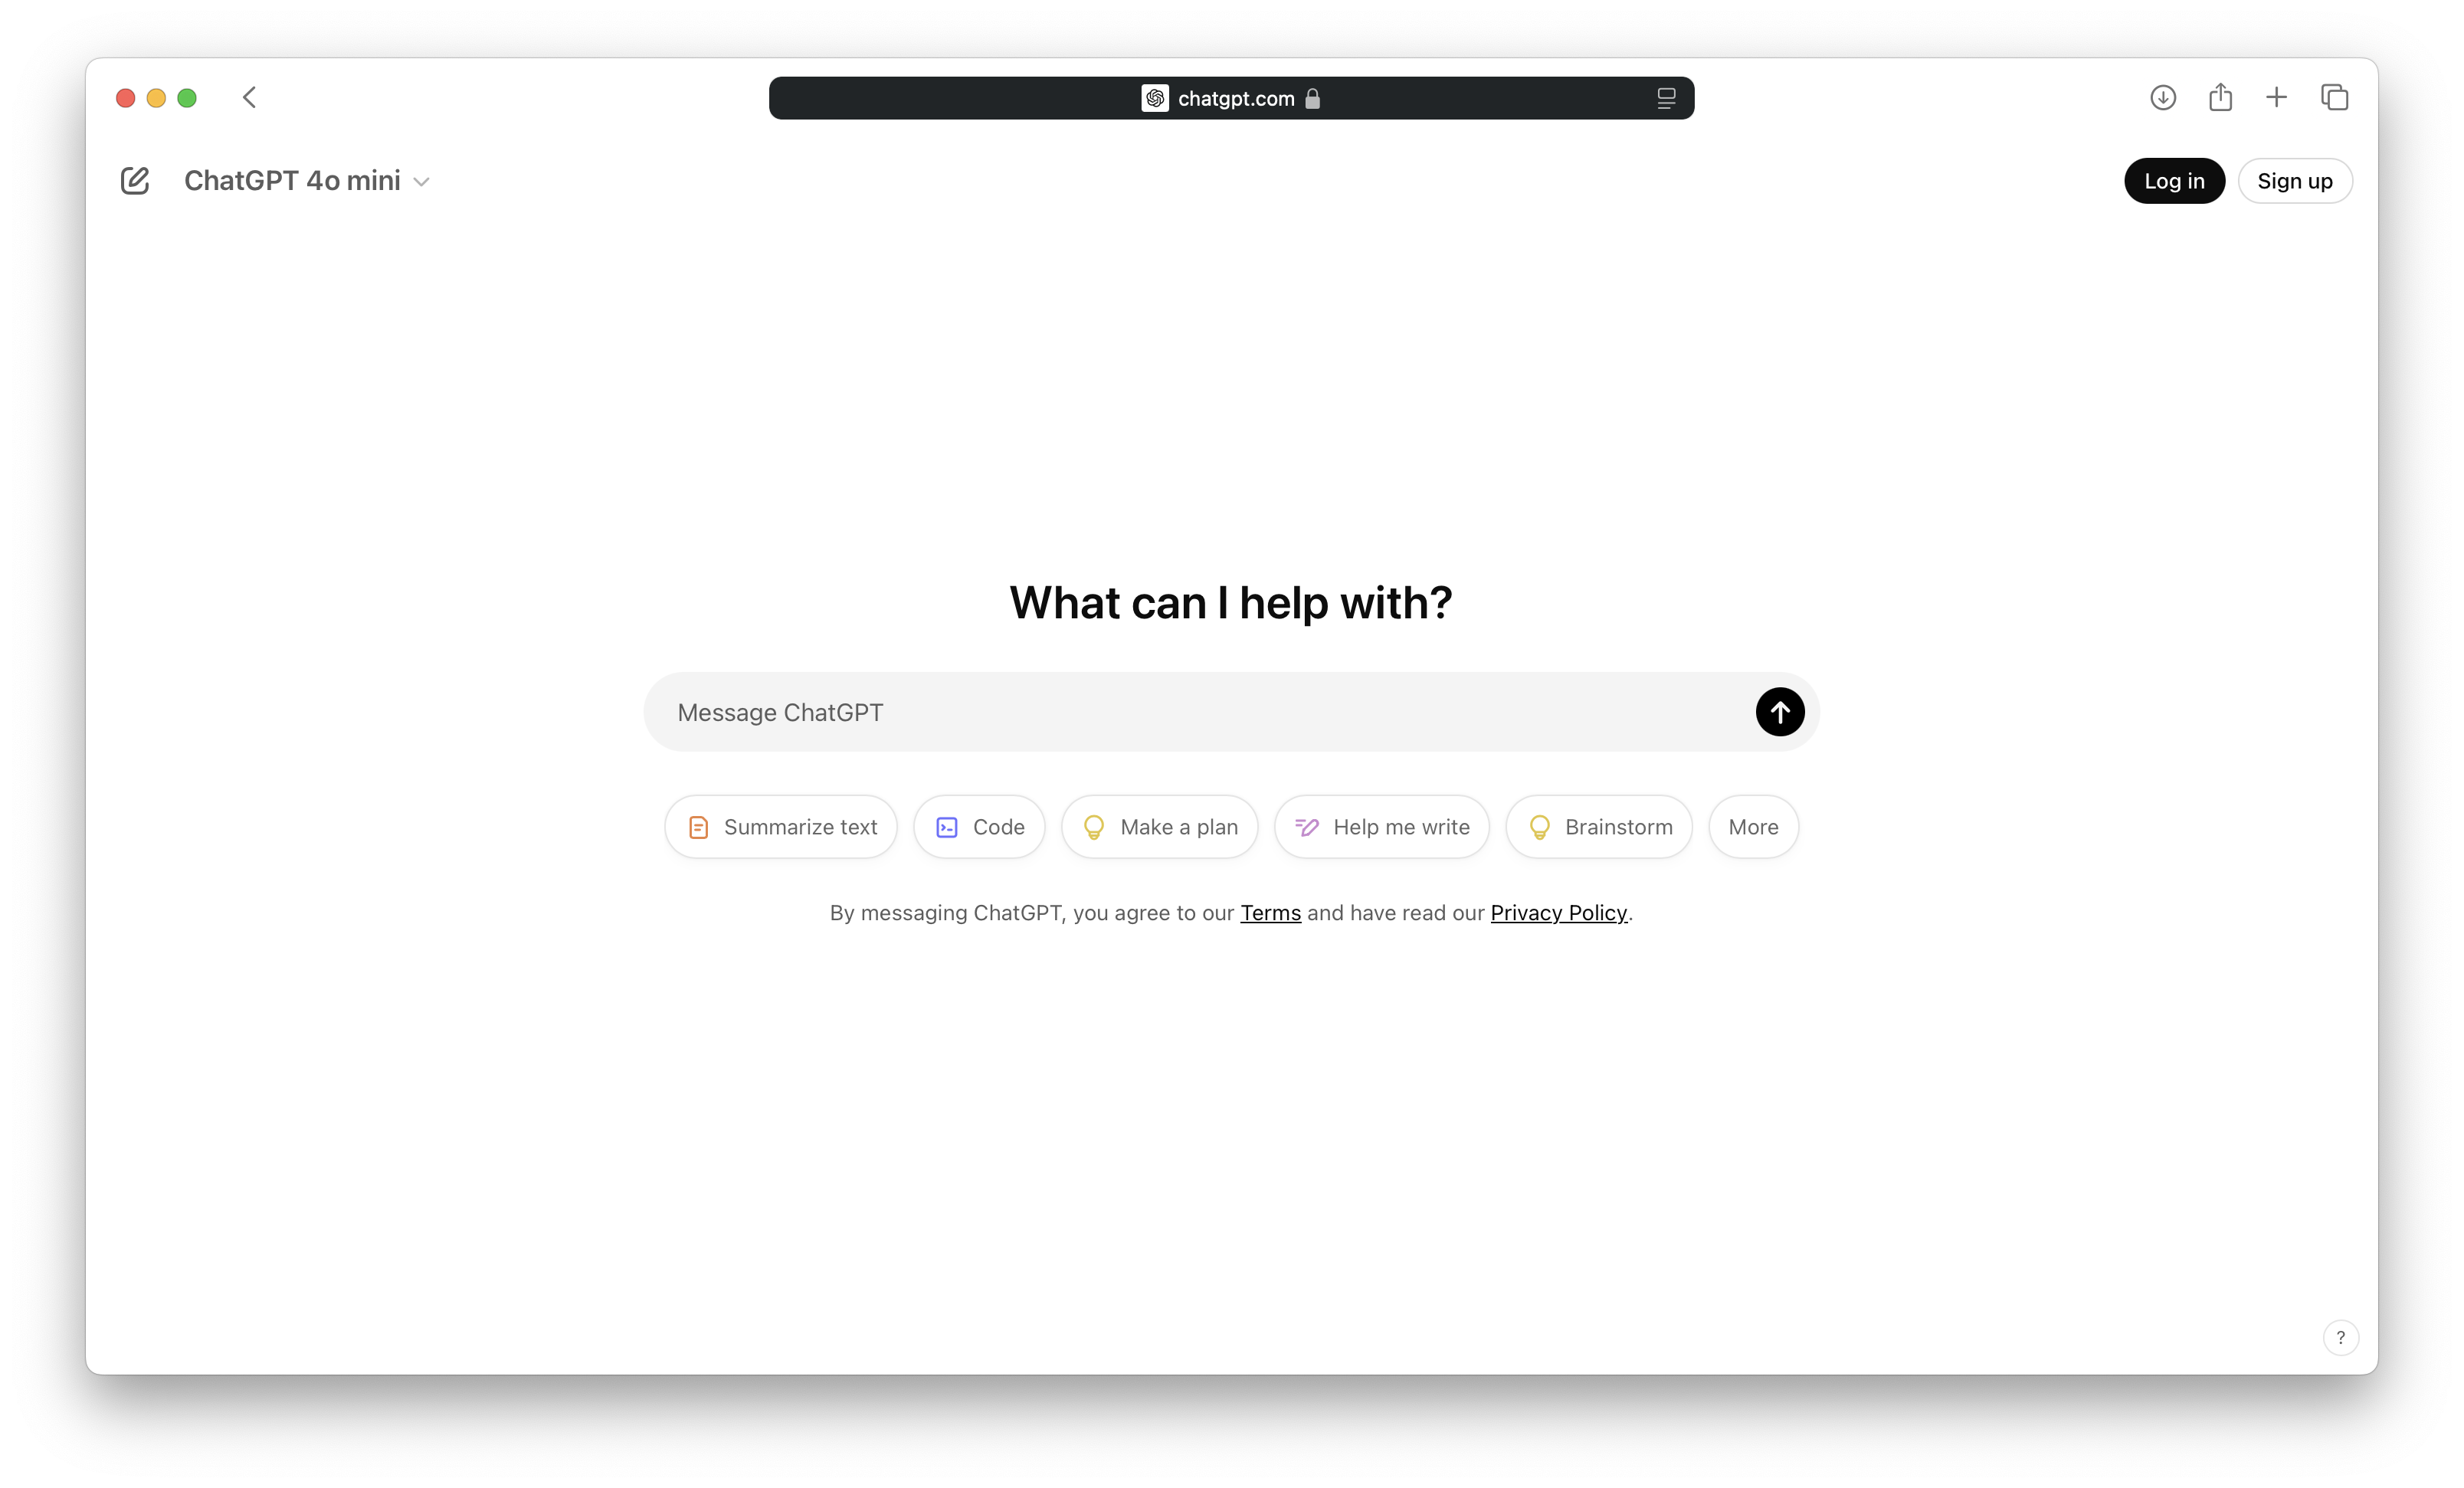
\includegraphics[width=0.8\textwidth]{pics/ChatGPT.png}
    \caption{\textsf{ChatGPT}的网站界面}
\end{figure}

经典原汁原味的\textsf{ChatGPT},笔者使用最多的模型。

\subsubsection*{\textsf{GPT}模型家族介绍}
\begin{itemize} 
    \item \textsf{GPT-4}: \textsf{OpenAI}推出的多模态语言模型,能够处理文本和图像输入,具备更强的推理能力,广泛用于复杂任务和专业应用。 
    \item \textsf{GPT-4-turbo (GPT-4o)}: 更加高效和优化的版本,提供\textsf{GPT-4}的核心能力,但在性能和计算成本上经过调整,响应速度更快,成本更低。 
    \item \textsf{GPT-4-turbo-mini (GPT-4o-mini)}: 轻量版的\textsf{GPT-4-turbo},专为对计算资源要求更低的场景设计,提供基本的语言生成能力,适合处理较轻量的任务。 
    \item \textsf{GPT-o1}: 专门优化的\textsf{GPT}系列模型,注重推理和问题解决能力,针对特定任务场景(如长文本处理或特定领域的应用)进行了定制。 
    \item \textsf{GPT-o1-mini}: \textsf{GPT-o1}的轻量版,针对资源受限环境下的自然语言处理任务提供快速响应,支持基础语言生成和理解任务。 
\end{itemize}

\subsection{\textsf{Claude}}
\roundedbox{\color{RedOrange}{\textsf{必须:}\hyperlink{warp}{\faIcon{globe}} \hyperlink{mail}{\faIcon{mail-bulk}}} \color{Melon}{\textsf{可选:}\hyperlink{google}{\faIcon{google}} \hyperlink{card}{\faIcon{credit-card}} \hyperlink{gift-card}{\faIcon{app-store-ios}}}}

\begin{quote}{续下文}
    \Huge{“}
    \normalsize \texttt{我觉得经典Claude(英语)的精英味最重,很多时候对引用边缘概念边缘梗,不会加以解释,说话的腔调
    有时候会像一个大西洋,滚石,连线,IGN这种类杂志媒体的编辑,这已经超过了普通人对常识和常用
    语的理解—它会认为,你在问我这个问题,那你一定是这个领域的爱好者,咱就不内行人说外行话
    了。经典Claude的音染比较明显,属于风格化调校。}
    \end{quote}

\textsf{Claude}由\textsf{Anthropic}公司开发,该公司与\textsf{OpenAI}构成了AI界的两家巨头。点击 \href{https://claude.ai}{\color{black}\faLink} 进入\textsf{Claude}的网站。此处可以使用\textsf{Google}帐号注册。
\textsf{Claude}有个\textsf{Artifacts}功能能实时预览代码效果,比如你在要求它做一个网页,它会把代码渲染出的页面给你看。\textsf{Claude}的淡米色背景笔者挺喜欢的。
\begin{figure}[H]
    \centering
    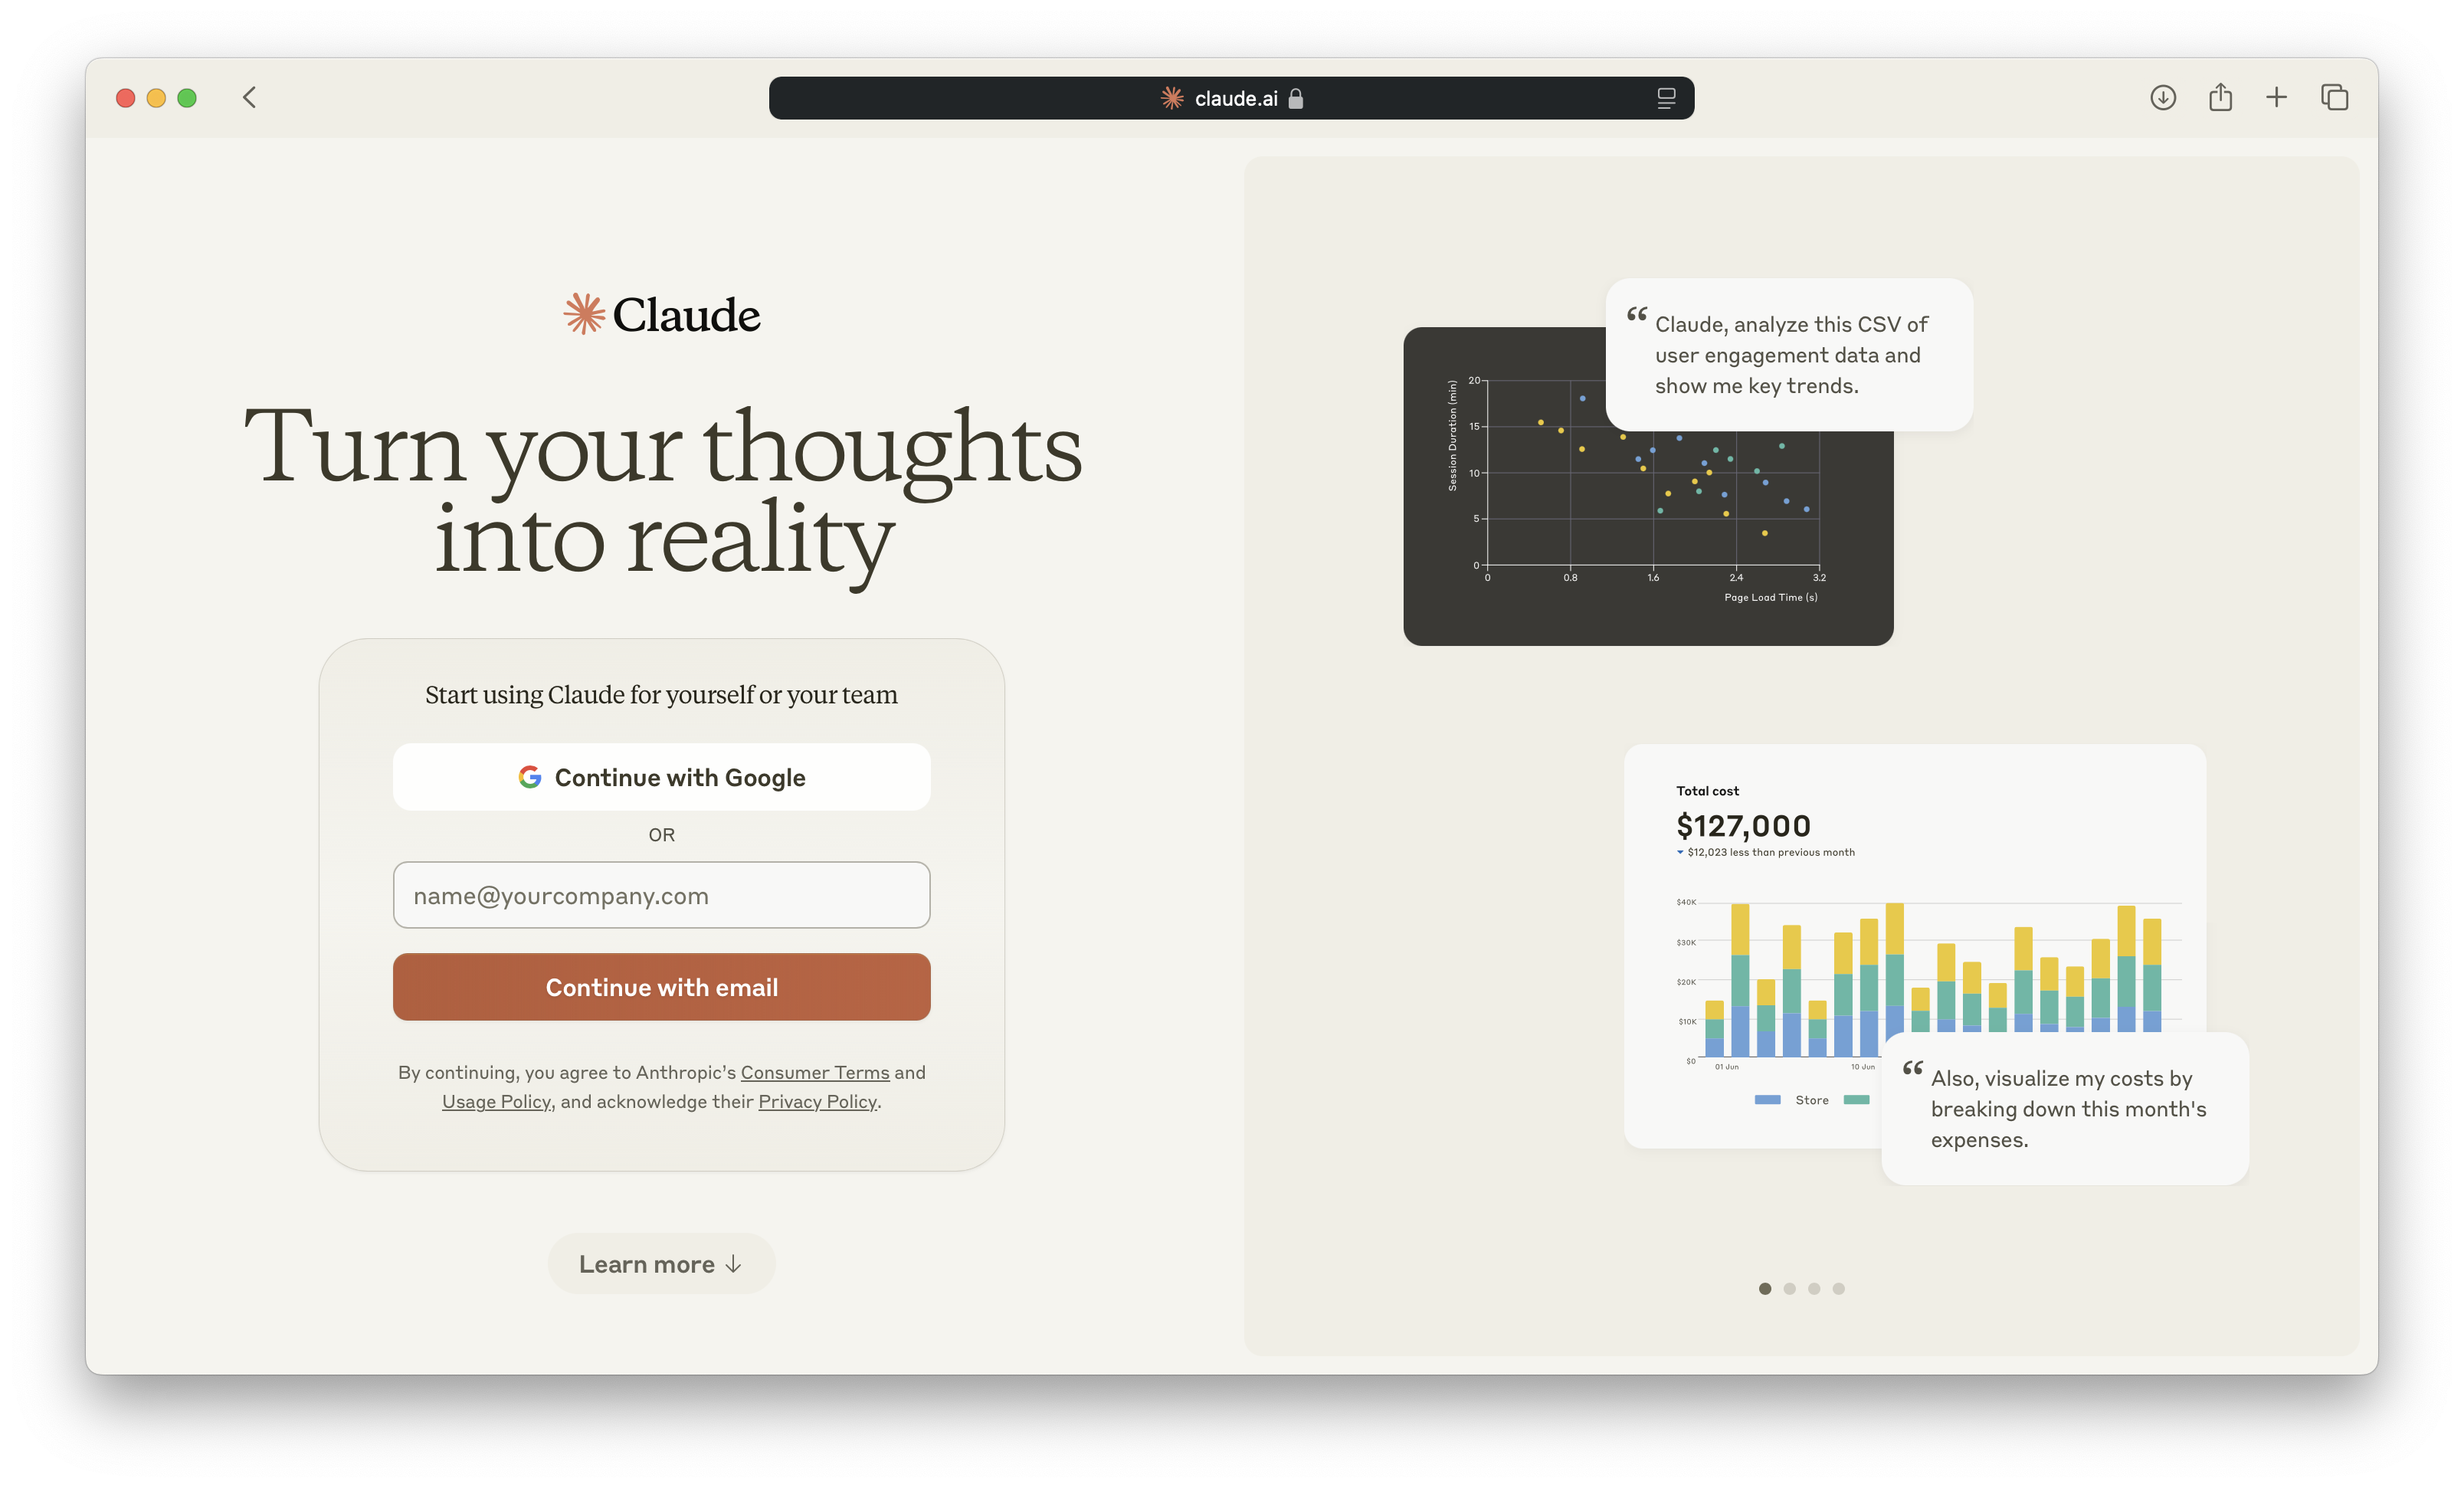
\includegraphics[width=0.8\textwidth]{pics/Claude.png}
    \caption{\textsf{Claude}的网站界面}
\end{figure}

\subsubsection*{\textsf{Claude}模型家族介绍}
\begin{itemize}
    \item \textsf{Claude 3 Haiku}: 最快速的模型,适合日常任务。
    \item \textsf{Claude 3 Opus}: 擅长写作和复杂任务的强大模型。
    \item \textsf{Claude 3.5 Sonnet}: \textsf{Anthropic}最智能的模型,具有卓越的综合能力。
\end{itemize}

\subsection{\textsf{Gemini}}
\roundedbox{\color{RedOrange}{\textsf{必须:}\hyperlink{warp}{\faIcon{globe}} \hyperlink{google}{\faIcon{google}}}}

\begin{quote}{续下文}
    \Huge{“}
    \normalsize \texttt{Gemini,Llama给人的感觉比较松散,他们似乎在以一个虚拟的平台用户作为对话对象,可能是偏小红书这个水平的用户,风格都比较活跃,Gemini会有点愤世嫉俗,有时候会对不公正,不科学的现象产生暴怒的情绪,Llama有点没心没肺。比较偏流行味的调校。}
    \end{quote}

如果之前登录过\textsf{Google}帐号,点击 \href{https://aistudio.google.com/app/prompts/new_chat}{\color{black}\faLink},应该能直接进入对话界面。右侧可以选择模型,我一般选择最强大的\textsf{Gemini 1.5 Pro 002}。
对于材料很长很长的场景,我都会选择\textsf{Gemini},因为免费额度很大,不用花钱。

\subsubsection*{\textsf{Gemini}模型家族介绍}
    \begin{itemize}
        \item \textsf{Gemini 1.5 Pro:}  针对复杂任务优化的更强大版本,具备高级推理、规划和理解能力。
        \item \textsf{Gemini 1.5 Ultra:}  规模最大、功能最强的 \textsf{Gemini} 模型,在各种基准测试中表现出色。
        \item \textsf{Gemini 1.5 Nano:}  专为移动设备设计的轻量级版本,可在设备上高效运行。
        \item \textsf{Gemini 1.5 Flash:} 专注于快速响应的小型 \textsf{Gemini} 模型,适用于对延迟敏感的应用。
    \end{itemize}

\subsection{其他模型}
\roundedbox{\color{RedOrange}{\textsf{必须:}\hyperlink{mail}{\faIcon{mail-bulk}}} \color{Melon}{\textsf{可选:}\hyperlink{warp}{\faIcon{globe}}}}

\begin{quote}{Trisimo崔思莫}
    \Huge{“}
    \normalsize \texttt{国内的LLM基本就是抄ChatGPT,也是问答机的调校,但它们预设的用户的心智会比较弱,没有
    ChatGPT的学术感,就随便答一下完事,最重要的是不挑战敏感内容,不要挑战领导,不要挑战体制,
    不要挑战“祖宗的好东西”,的确大部分用国产AI的人,对输出也没有多大追求,就是听个响,又不是没反应。}
    \end{quote}



\textsf{Deepseek} \href{https://www.deepseek.com}{\color{black}\faLink} 属于国产模型里做得不错的,API价格很便宜。

\roundedbox{\color{RedOrange}{\textsf{必须:}\hyperlink{warp}{\faIcon{globe}} \hyperlink{mail}{\faIcon{mail-bulk}}}}

\textsf{Llama3.1} \href{https://huggingface.co/chat/}{\color{black}\faLink} \textsf{Meta}公司制作的开源模型。

\textsf{Qwen2.5} \href{https://huggingface.co/chat/}{\color{black}\faLink} 阿里巴巴公司制作的开源的模型,水平也不错,从\textit{杭州级}走向了\textit{加州级}(笑)。
注意,以上两个模型的链接都指向\textsf{HuggingChat},进入之后需要手动选择。

主流的大模型就介绍这么多。




\section{AI工具的使用}

\subsection{AI搜索工具}
\roundedbox{\color{RedOrange}{\textsf{必须:}\hyperlink{warp}{\faIcon{globe}} \hyperlink{mail}{\faIcon{mail-bulk}} \color{Melon}{\textsf{可选:}\hyperlink{google}{\faIcon{google}} \hyperlink{card}{\faIcon{credit-card}}}}}

\textsf{Felo.ai} \href{https://felo.ai/search}{\color{black}\faLink} 
和 \textsf{Perplexity} \href{https://www.perplexity.ai}{\color{black}\faLink} 都是很好的AI搜索工具,适合需要事实的场景。
两者都可以使用\textsf{Google}帐号登录。笔者更喜欢使用\textsf{Felo},因为每天有一些免费使用pro搜索的额度,而且效果比\textsf{Perplexity}好。

\subsubsection{代码专精型搜索工具}
\roundedbox{\color{RedOrange}{\textsf{必须:}\hyperlink{warp}{\faIcon{globe}} \hyperlink{mail}{\faIcon{mail-bulk}} \color{Melon}{\textsf{可选:}\hyperlink{google}{\faIcon{google}} \hyperlink{github}{\faIcon{github}} \hyperlink{card}{\faIcon{credit-card}}} \faIcon{alipay}}}

\textsf{Devv.ai} \href{https://devv.ai}{\color{black}\faLink} 可使用\textsf{Google}帐号或\textsf{Github}帐号登录。

\subsection{AI驱动的代码编辑器}
\roundedbox{\color{RedOrange}{\textsf{必须:}\hyperlink{warp}{\faIcon{globe}} \hyperlink{mail}{\faIcon{mail-bulk}} \color{Melon}{\textsf{可选:}\hyperlink{card}{\faIcon{credit-card}}} \hyperlink{api}{\faIcon{code}}}}

\textsf{Cursor} \href{https://www.cursor.com}{\color{black}\faLink} 是一款AI代码编辑器,热度很高,但是笔者没有深度使用过。据说可以解析一整个项目的所有代码,并且你说几句话就能给你写出一个应用来。感兴趣的可以试试。

\hypertarget{api}{\section{模型的API调用方法}}
如果你想使用一些\textsf{OpenAI},\textsf{Anthropic}只提供给付费用户的高级模型,但又不想花每月\$20的订阅费,那么你就可以尝试通过API调用。

\subsection{API供应商}
\roundedbox{\color{RedOrange}{\textsf{必须:}\hyperlink{warp}{\faIcon{globe}} \hyperlink{mail}{\faIcon{mail-bulk}} \faIcon{alipay}}}

\textsf{luee.net} \href{https://luee.net}{\color{black}\faLink} 是笔者使用的一家供应商,可以使用支付宝支付。充值后在API KEY页面可以新建API Key,API Key就是用来调用模型的密钥。
新建Key的时候会让你选择可以使用的模型,如果你不清楚自己想要什么,那就全选好了。笔者勾选了\textsf{gpt-4o}, \textsf{chatgpt-4o-latest}, 
\textsf{claude-3-opus-20240229}, \textsf{claude-3-5-sonnet-20240620}和\textsf{o1-preview}这几个模型。
\subsection{API的使用方法}
\textsf{Nextchat} \href{https://app.nextchat.dev}{\color{black}\faLink} 允许你填入你自己的API并进行对话。点击界面左下角的齿轮图标进入设置,向下滚动找到“Custom Endpoint”,
    在“OpenAI Endpoint”处填入\texttt{https://api.luee.net}(此处以上文提到供应商为例;其他供应商操作也大同小异),并在下面的 “API KEY”一栏中填入你刚才创建的密钥。在下面的"Model"处可以选择你默认想要的模型。

    如果你想要使用\textsf{Anthropic}的模型,那就在上面的“Model Provider”选单中选择\textsf{Anthropic},填入相关内容,其余同理。

现在关闭设置界面,就可以开始对话了。其他功能不多赘述,大家可以自行探索。

\section{在本地运行语言模型}
\subsection{模型知识科普}
如果你去观察,可以发现市面上有各种不同的模型。\textsf{llama3.2},\textsf{llama3.1},\textsf{qwen2.5},\textsf{deepseek-coder-v2},\textsf{command-r-plus}\dots
简直要挑花眼了!而且每种模型可能还有\ “8B”\ \ “70B”\ \ “405B”\ 之类的版本。
有小朋友可能会问,这里的“B”是什么意思呢?其实“B”代表“billion”,即10亿。此处是参数量——模型中“参数”的数量。因此:
\begin{itemize}
    \item 7B = 7 billion = 70亿个参数
    \item 70B = 70 billion = 700亿个参数
    \item 400B = 400 billion = 4000亿个参数
\end{itemize}

参数是模型学习到的权重,用来表示输入和输出之间的关系。模型的参数越多,它能够学习和捕捉的复杂信息就越丰富。

举个简单的类比,可以把语言模型想象成一个大脑,更多的参数意味着模型更“聪明”,能够处理更复杂的任务,
理解更细微的语言差异。比如,一个7B参数的模型可能能够生成基本的对话,但可能在处理深层次推理或非常专业化的任务时显得力不从心。
而70B或400B参数的模型,则可能能够更好地理解上下文,生成更准确或自然的内容。例如,初代GPT-4,就被猜测有超过1800B的参数。

\subsection{\textsf{Ollama}}
\roundedbox{\color{RedOrange}{\textsf{必须:}\hyperlink{warp}{\faIcon{globe}}}}

如果你对在自己的设备上运行LLM感兴趣,那么你可以尝试\textsf{Ollama} \href{https://ollama.com}{\color{black}\faLink}。
下载并安装对应你设备的版本后,就可以在终端(Terminal)上使用了。你可以在模型仓库 \href{https://ollama.com/library}{\color{black}\faLink} 
找到你想要的模型。比如,在终端输入\texttt{ollama run qwen2.5}就是下载并运行7B的\textsf{Qwen}模型(如果你之前没有运行过这条命令)。

一般而言,7B参数的语言模型在4-bit量化下4.7GB。如果你的设备有GPU,特别是\textsf{NVIDIA}的GPU,且显存大于模型的大小,
那么推理时就可以享受到显著的加速。\textsf{AMD}的\textsf{ROCm}支持的GPU和\textsf{Apple Silicon}的\textsf{Metal}也能提供加速。
\subsection{其他本地运行模型的方法}
\roundedbox{\color{RedOrange}{\textsf{必须:}\hyperlink{warp}{\faIcon{globe}}}}

除了\textsf{Ollama},也有\textsf{LM Studio} \href{https://lmstudio.ai}{\color{black}\faLink} 之类的软件可以使用。如果你觉得\textsf{Ollama}不足以满足你的需求可以试试。

\section{一些实用技巧}
\hypertarget{sms-code}{\subsection{接码平台}}
\roundedbox{\color{RedOrange}{\textsf{必须:}\hyperlink{warp}{\faIcon{globe}} \hyperlink{mail}{\faIcon{mail-bulk}} \faIcon{alipay}} \color{Melon}{\textsf{可选:}\hyperlink{card}{\faIcon{credit-card}}}}

\textsf{Sms-activate} \href{https://sms-activate.io/cn}{\color{black}\faLink} 可获取可用的手机号并接收验证码。
(这个网站是从俄文机翻过来的,所以有些地方可能很生硬。而且网页的加载速度也不快,操作时需要有耐心。)

\hypertarget{card}{\subsection{虚拟信用卡}}
\roundedbox{\color{RedOrange}{\textsf{必须:}\hyperlink{warp}{\faIcon{globe}} \hyperlink{mail}{\faIcon{mail-bulk}} \faIcon{alipay}}}

虚拟信用卡允许你支付美元来订阅各种服务,比如\textsf{ChatGPT Plus}或者使用\textsf{OpenAI}官方的API。
你可以自行搜索或者前往\textsf{Wildcard} \href{http://bewildcard.com/}{\color{black}\faLink} 查看。

\section{Scientific 上网(其二)}
上文中提了如何在电脑端科学上网,这里来讲一下其他平台的方法。笔者认为,在所有设备上都部署代理软件是必要的。这样可以获得统一的体验,最大程度远离那些不堪入目的网站。
\subsection{\textsf{Android}端}
\roundedbox{\color{RedOrange}{\textsf{必须:}\hyperlink{warp}{\faIcon{globe}}}}

在\textsf{Android}上,你可以使用\textsf{ClashMetaForAndroid} \href{https://github.com/MetaCubeX/ClashMetaForAndroid/releases/tag/v2.11.1}{\color{black}\faLink} ,选择对应版本下载安装即可。
如果你不确定要下哪个,那就下载带有“Universial”字样的版本。当然,你也可以问语言模型。
\subsection{\textsf{iOS}端}
\roundedbox{\color{RedOrange}{\color{Melon}{\textsf{可选:}\hyperlink{gift-card}{\faIcon{app-store-ios}}} \hyperlink{card}{\faIcon{credit-card}}}}

\textsf{iOS}端略复杂,你首先需要一个非国区(比如美区)的\textsf{Apple Account}。你可以前往 \href{https://icloud.com}{\color{black}\faLink} 注册一个,网上有不少相关的教程。

注册完成后,你还需要代理软件。然而\textsf{iOS}上不少代理软件都需要付费,例如\textsf{Shadowrocket}/\textsf{Quantumult X}/\textsf{Surge}/\textsf{Loon}等。不过也有免费的,比如\textsf{Potatso Lite}。

如果你有意付费,但又没有支付方法,可以试试礼品卡 \hyperlink{gift-card}{\faIcon{share}} 。当然你也可以使用虚拟卡 \hyperlink{card}{\faIcon{share}} 。
\hypertarget{gift-card}{\subsubsection*{礼品卡支付方法(美区)}}
打开支付宝,搜索“\textsf{pockytshop}”,进入小程序,找到\textsf{Apple Gift Card US},购买并在\textsf{App Store}中兑换即可。现在就可以购买\textsf{App Store}中的应用了。

\subsection{给你的路由器装上代理}
想要代理的终极体验吗?那就给你的路由器装上代理吧。你可以搜索相关内容或者\textsf{OpenClash}自行操作。

\section{推荐的工具}
\begin{itemize}
    \item 浏览器:\textsf{Safari} \href{https://www.apple.com/safari/}{\color{black}\faLink} 适用于\textsf{Apple}设备,耗电较少;
    \textsf{Chrome} \href{https://www.google.com/chrome/}{\color{black}\faLink} 由\textsf{Google}出品,是最流行的浏览器之一;
    \textsf{Firefox} \href{https://www.mozilla.org/en-US/firefox/}{\color{black}\faLink} 适合那些讨厌\textsf{Chrome}的人;
    \textsf{Arc Browser} \href{https://arc.net}{\color{black}\faLink} 是个新东西,如果你想尝试垂直标签页可以试试。
    \item 文字编辑器:\textsf{Visual Studio Code} \href{https://code.visualstudio.com}{\color{black}\faLink} ,大名鼎鼎的\textsf{VSCode},由微软开发,适合各类文字编辑任务。装上对应插件后还可以写各种编程语言的项目。
    \item 通讯工具:\textsf{Telegram} \href{https://telegram.org}{\color{black}\faLink} ,流畅清爽,你可以在许多\textsf{Github}项目的页面上看到\textsf{Telegram}的讨论群组。缺点是注册时可能要一番功夫。
    \item 社交平台:\textsf{X(Twitter)} \href{https://x.com/}{\color{black}\faLink} :如果你对AI感兴趣,可以不夸张地说这上面有最好的中文的,AI内容交流氛围。此处有一些分享 \href{https://www.aisourcehub.info}{\color{black}\faLink}。
    \item 笔记软件:\textsf{Obsidian} \href{https://obsidian.md}{\color{black}\faLink} ,本地存储的笔记软件。只要你保管得当,永远不会有丢失数据之虞。\sout{点名批评Notion}
    \item 排版工具:\LaTeX\ \href{https://www.latex-project.org}{\color{black}\faLink} ,还在为Word格式调整而抓狂吗?赶紧来试试\LaTeX 吧!本文便是由\LaTeX 写就。这里有一份简洁的介绍 \href{https://github.com/stone-zeng/latex-talk}{\color{black}\faLink}。
\end{itemize}
